\documentclass[12pt,a4paper]{article}
 
%encoding
%--------------------------------------
\usepackage[utf8]{inputenc}
\usepackage[T1]{fontenc}
%--------------------------------------
 
%Portuguese-specific commands
%--------------------------------------
\usepackage[portuguese]{babel}
%--------------------------------------
 
%Hyphenation rules
%--------------------------------------
\usepackage{hyphenat}
\hyphenation{mate-mática recu-perar}
%--------------------------------------

\usepackage{graphicx}
\graphicspath{ {images/} }
\usepackage{caption}
\usepackage{subcaption}
\usepackage{amsmath}

\begin{document}

\begin{titlepage}

\newcommand{\HRule}{\rule{\linewidth}{0.5mm}} % Defines a new command for the horizontal lines, change thickness here

\center % Center everything on the page
 
%----------------------------------------------------------------------------------------
%	HEADING SECTIONS
%----------------------------------------------------------------------------------------

\textsc{\LARGE INSTITUTO SUPERIOR DE \\[0.2cm] ENGENHARIA DE LISBOA}\\[0.5cm]
\textsc{\LARGE ADEETC  }\\[0.3cm]
\textsc{\Large Licenciatura em Engenharia Informática e Multimédia }\\[0.3cm]
\textsc{\Large Semestre de Verão}\\[0.5cm]
\textsc{\Large 2º Trabalho Prático}\\[0.5cm]

%----------------------------------------------------------------------------------------
%	TITLE SECTION
%----------------------------------------------------------------------------------------

\HRule \\[0.4cm]
{ \huge \bfseries Codificação de Sinais Multimédia}\\[0.03cm] % Title of your document
\HRule \\[1.5cm]

%----------------------------------------------------------------------------------------
%	AUTHOR SECTION
%----------------------------------------------------------------------------------------
\Large \emph{Realizado por:}\\
João \textsc{Santos} nº 39348\\ 
Rui \textsc{Santos} nº 39286\\[2cm] 
%----------------------------------------------------------------------------------------
%	DATE SECTION
%----------------------------------------------------------------------------------------

{\large Abril, 2017}\\[1cm]

%----------------------------------------------------------------------------------------
%	LOGO SECTION
%----------------------------------------------------------------------------------------


\includegraphics[scale=0.3]{iselLogo.jpg}\\[1cm]
 
%----------------------------------------------------------------------------------------
\vfill % Fill the rest of the page with whitespace
\end{titlepage}

%-------------------------------------------------------
\tableofcontents
\newpage
\listoffigures
\listoftables
\newpage
%-------------------------------------------------------
\section{Introdução}
O segundo trabalho prático da disciplina de CSM (Codificação de Sinais Multimédia) tem como objetivo a exploração dos conceitos de compressão de dados sem perdas baseados na teoria da informação.\\ Foi utilizado o algoritmo de \textit{Huffman} no trabalho prático para obter uma codificação sem perdas. Foram implementadas várias funções que permitiram realizar o trabalho e que vão ser descritas mais à frente. Para testar a robustez do algoritmo foram utilizados vários tipos de média, tais como, imagens, texto (txt e pdf), audio (mp3), midi e um ficheiro com extensão .txt que contem um ecg (eletrocardiograma). Com os algoritmos necessários desenvolvidos e testados foi realizado o cálculo da entropia e a interpretação dos resultados obtidos.\\ Finalmente houve uma comparação entre os ficheiros codificados e descodificados, sendo que, o objetivo é que ambos os ficheiros sejam idênticos pois a compressão implementada é \textit{lossless} (sem perdas).
\newpage
\section{Desenvolvimento}
A fase de desenvolvimento do trabalho conta com a compreensão do algoritmo de \textit{Huffman} e um estudo sobre o modo mais eficiente de desenvolver os métodos necessários. Para que o compressor seja bem desenvolvido foi pedido no enunciado do trabalho a implementação dos seguintes métodos:
% LISTA DOS MÉTODOS
\begin{enumerate}
\item função \textbf{gera\_huffman()} que gera uma tabela com o código binário para cada símbolo de um dado conjunto, usando o método de \textit{Huffman}. Esta função tem como parâmetros de entrada um conjunto de símbolos e o número de ocorrências de cada símbolo, dado pelo seu histograma.
\item função \textbf{codifica}() que dada uma mensagem (sequência de símbolos) e a tabela da ponto anterior,
retorne uma sequência de bits com a mensagem codificada.
\item função \textbf{descodifica()} que dada uma sequência de bits (mensagem codificada) e a tabela do ponto 1, retorne uma sequência de símbolos (mensagem descodificada).
\item função \textbf{escrever()} que dada uma sequência de bits (mensagem codificada) e o nome do ficheiro,
escreva a sequência de bits para o ficheiro.
\item função \textbf{ler()} que dado o nome do ficheiro, leia uma sequência de bits (mensagem codificada) contida no ficheiro.
\end{enumerate}

Podemos observar na figura 1 um diagrama com o fluxo de ocorrências do programa desenvolvido.

\begin{figure}[h]
\centering
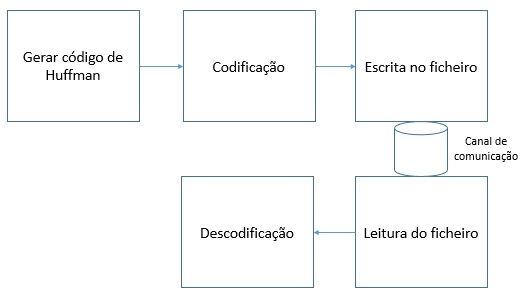
\includegraphics[width=.7\linewidth]{diagrama.jpg}
\caption{Diagrama do compressor de Huffman.}
\end{figure}

% FIM DA LISTA DOS MÉTODOS
\subsection{Algoritmo de Huffman}
A codificação de \textit{Huffman} é um método de compressão que utiliza as probabilidades de ocorrência dos símbolos no conjunto de dados a comprimir, de modo, a determinar códigos de comprimento variável (VLC) para cada símbolo. Este algoritmo é utilizado na compressão JPEG e MPEG.
\subsubsection{Algoritmo de codificação de Huffman}
O modo de funcionamento do algoritmo é o seguinte:
% LISTA DO FUNCIONAMENTO DO CÓDIGO DE HUFFMAN
\begin{enumerate}
\item \textbf{Ordenar} os símbolos de acordo com a respetiva frequência de ocorrência ou probabilidade.
\item Aplicar, de forma recursiva, um processo de \textbf{contração} aos dois símbolos com menor probabilidade, obtendo-se um novo símbolo cuja probabilidade é igual à soma das probabilidades dos símbolos que lhe deram origem, repetindo-se esta contração até que todos os símbolos tenham sido contraídos em \textbf{um} único símbolo com probabilidade igual a 1.
\end{enumerate}
% FIM DA LISTA
Para uma melhor compreensão do algoritmo de \textit{Huffman} podemos utilizar a tabela exemplo 1 com os seguintes símbolos e ocorrências:
\newline
% ÍNICIO DA TABELA DE EXEMPLO
\begin{table}[h]
\centering
\label{my-label}
\begin{tabular}{|c|c|}
\hline
Símbolo & Ocorrência \\ \hline
A       & 24         \\ \hline
B       & 12         \\ \hline
C       & 10         \\ \hline
D       & 8          \\ \hline
E       & 8          \\ \hline
\end{tabular}
\caption{Tabela exemplo.}
\end{table}

% FIM DA TABELA EXEMPLO
Partindo da tabela 1 é possível representar em forma de árvore os símbolos e as suas ocorrências, obtendo a figura 2.
\newpage
\begin{figure}[h]
\centering
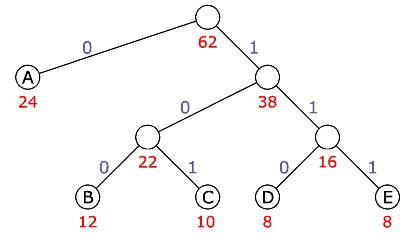
\includegraphics{arvore.jpg}
\caption{Árvore de código de acordo com Huffman.}
\end{figure}

Como é possível observar através do diagrama em árvore os símbolos com maior número de ocorrências vão ser codificados com menor número de bits, para este exemplo o caso mais percetível é o símbolo \textit{A} que é codificado com apenas um bit. Com a árvore desenvolvida e os bits atribuídos a codificação final de cada símbolo estão representados na tabela 2.

% ÍNICIO DA TABELA FINAL
\begin{table}[h]
\centering
\label{my-label}
\begin{tabular}{|c|c|c|c|}
\hline
Símbolo & Ocorrência & Código & Tamanho do código \\ \hline
A       & 24         & 0      & 1                 \\ \hline
B       & 12         & 100    & 3                 \\ \hline
C       & 10         & 101    & 3                 \\ \hline
D       & 8          & 110    & 3                 \\ \hline
E       & 8          & 111    & 3                 \\ \hline
\end{tabular}
\caption{Tabela final da codificação de Huffman.}
\end{table}
% FIM DA TABELA FINAL

Supondo agora, por exemplo, que a mensagem a codificar, é a sequência "ABADE", esta mensagem codificada com a técnica de \textit{Huffman} resulta na seguinte sequência de 11 bits:
\begin{center}
   01000110111
   \end{center} 
\newpage
\subsubsection{Descodificação de Huffman}
Para ilustrar o algoritmo de \textbf{descodificação de bits em série} retome-se o exemplo da figura 1, assumindo que a tabela de codificação binária já se encontra disponível no lado do descodificador.\\
A descodificação de \textit{Huffman} baseado no algoritmo de descodificação de bits em série consiste nos seguintes passos:
\begin{enumerate}
\item Ler o fluxo de bits comprimidos, \textbf{bit após bit}, e percorrer a tabela até que se encontre uma ocorrência.
\item À medida que cada bit é utilizado, deverá ser \textbf{descartado}. Quando existe uma ocorrência, o descodificador de \textit{Huffman} coloca na saída o \textbf{símbolo} correspondente à entrada da tabela, completando a descodificação do símbolo atual.
\item Repetir os passos 1 e 2 até que o fluxo comprimido tenha sido consumido.
\end{enumerate}

\subsection{Escrita e Leitura em ficheiro}
De modo a simular um canal de comunicação foram desenvolvidos os métodos \textit{escrever()} e \textit{ler()}, como os nomes indicam permitem a escrita e leitura num ficheiro de extensão .txt.

\subsubsection{Escrita}
O método escrever é um método que passados como argumentos uma sequência de bits (mensagem codificada) e o nome do ficheiro, escreve a sequência de bits para esse ficheiro.\\ A solução implementada neste método tem quatro pontos fundamentais, dos quais:
\begin{enumerate}
\item Realizar um \textit{reshape} na mensagem recebida de modo a agrupar os bits de 8 em 8.
\item Com os bits agrupados de 8 em 8 realizamos uma transformação de valores binários para inteiros.
\item Com a lista de inteiros é realizada uma transformação para caracteres.
\item Escrita dos caracteres no ficheiro.
\end{enumerate}

\subsubsection{Leitura}
O método de leitura \textit{ler()} faz exatamente o oposto ao método de escrita, ou seja, dado o nome do ficheiro, é lida a sequência de caracteres (mensagem codificada) contida no ficheiro e transformada para uma mensagem binária.\\ A solução encontrada para este método tem os seguintes pontos fundamentais:
\begin{enumerate}
\item Leitura dos caracteres do ficheiro.
\item Conversão de caracteres para números inteiros.
\item Conversão de inteiros para binário.
\end{enumerate}

\subsection{Resultados obtidos}
Com todas as funções desenvolvidas é nos pedido no enunciado do trabalho a realização de cálculos e a medição de tempos de processamento de modo a testar o algoritmo. Os pontos pedidos são os seguintes:\\
\newline
a) Gerar o código usando a função \textbf{gera\_huffman()}. Medição do tempo que demora a função.\\
\newline
b) Medição da entropia e o número médio de bits por símbolo. Calculo da eficiência.\\
\newline
c) Codificação da mensagem contida no ficheiro (usando a função \textbf{codifica()}). Medição do tempo
que a função demora a fazer a codificação.\\
\newline
d) Gravação de um ficheiro com a mensagem codificada, usando a função \textbf{escrever()}. Calculo do tamanho do ficheiro.\\
\newline
e) Ler do ficheiro o conjunto de bits, usando a função \textbf{ler()}.\\
\newline
f) Descodificação da mensagem (usando a função \textbf{descodifica()}) Medição do tempo que a função
demora a fazer a descodificação.\\
\newline
g) Comparação da mensagem descodificada com a original e verificar que são iguais (erro nulo).\\

\subsubsection{Tempos de processamento}
Os tempos de processamento são obtidos utilizando a biblioteca \textit{time} e são calculados do seguinte modo:\\
\newline
tempo1 = time()\\
funcao()\\
tempo2 = time()\\
tempo\_processamento = tempo2 - tempo1\\

Podemos observar na tabela 3 os tempos de processamento obtidos para cada função desenvolvida e o tempo total do algoritmo.

% ÍNICIO DA TABELA DE TEMPOS
\begin{table}[h]
\centering
\label{my-label}
\begin{tabular}{|c|c|c|c|}
\hline
Função & Tempo de processamento (\textit{segundos})\\
\hline
gera\_huffman() & 0.003 \\ 
\hline
codifica()      & 0.220 \\ 
\hline
escrever()      & 2.299 \\ 
\hline
ler()           & 0.301 \\
\hline
descodifica()   & 12.730\\
\hline
Tempo total     & 15.559\\
\hline
\end{tabular}
\caption{Tabela com os tempos de processamento.}
\end{table}
% FIM DA TABELA DE TEMPOS

Como se pode observar a partir da tabela 3 os tempos de processamento são relativamente baixo, exceto, o do descodificador. Isto deve-se ao facto de ser necessário realizar uma comparação bit a bit da mensagem e verificar se esse valor binário existe na tabela. O tempo total de processamento ronda os 15 segundos primeiramente devido ao tempo do descodificador.

\subsubsection{Entropia}
A entropia pode ser pode ser definida como o número médio mínimo de \textit{bits} necessário à representação de cada símbolo (\textit{$S_i$}) de uma dada fonte (\textit{$S$}) em função da probabilidade de ocorrência desse símbolo na fonte. Logo, a entropia é tanto maior quanto mais a incerteza. Podemos observar a fórmula utilizada para calculo da entropia em baixo.
\begin{center}
$H(S) = -\sum\limits_{i=1}^N p(s_i)\log_2p(s_i)$
\end{center}
Como o código de Huffman respeita, a entropia da fonte, os símbolos com maior probabilidade serão codificados com menos bits e os símbolos menos recorrentes serão codificados com mais \textit{bits}, pelo que o código final resultante é, em média, muito menor do que a fonte.

\subsubsection{Número médio de bits}
De seguida foi realizado o calculo do número médio de \textit{bits} por símbolo, como o nome indica, é uma média do número de \textit{bits} necessários para codificar cada símbolo. Podemos observar a formula utilizada para o calculo do número médio de \textit{bits} em baixo.
\begin{center}
$L = \sum\limits_{i=1}^N p(s_i)L(s_i)$
\end{center}

\subsubsection{Eficiência}
Por último com a entropia e o número médio de bits por símbolo calculados é possível calcular a eficiência do código através da seguinte fórmula.
\begin{center}
$\eta = \frac{H(S)}{L}$
\end{center}
O teorema de codificação de fonte de \textit{Shannon} diz que é possível codificar uma fonte, sem perdas, com um número médio de bits por símbolo maior ou igual à entropia da fonte:
\begin{center}
$H(S) < L < H(S) + \delta$
\end{center}
Assim, a codificação entrópica, consiste em codificar uma fonte de forma a atingir um número médio de bits por símbolo igual à entropia dessa fonte. 

\subsubsection{Valores obtidos}
% ÍNICIO DA TABELA DE VALORES
\begin{table}[h]
\centering
\label{my-label}
\begin{tabular}{|c|c|}
\hline
Entropia              & 7.445 \\ 
\hline
Nº médio de bits      & 7.467 \\ 
\hline
Eficiência            & 0.996 \\ 
\hline
\end{tabular}
\caption{Tabela com os valores obtidos.}
\end{table}
% FIM DA TABELA DE VALORES

Como referido anteriormente o valor da entropia e do número médio de \textit{bits} por símbolo deve ser igual à entropia. Observando os valores obtidos podemos deduzir que isto se confirma. Como a eficiência do código é a divisão entre estes dois valores e estes são quase idênticos é esperado uma eficiência de código com valor aproximado de 1 que vai de acordo com o resultado obtido.

\subsubsection{Ficheiros obtidos}
Por fim resta representar a comparação dos ficheiros antes e depois da descodificação. Visto ser uma técnica de compressão sem perdas os tamanhos dos ficheiros devem ser idênticos e a sua taxa de compressão deve dar uma valor igual a 1. A taxa de compressão é dada pela expressão:

\begin{center}
$\text{Taxa de Compressão} = \frac{\text{Imagem Original}}{\text{Imagem Descodificada}}$
\end{center}

Utilizando a biblioteca \textbf{path} e o método \textit{getsize()} dessa mesma biblioteca conseguimos obter os tamanhos das imagens originais e descodificadas, respetivamente. Através dos resultados obtidos podemos calcular a Taxa de Compressão utilizando a expressão descrita em cima. É possível observar na tabela 5 os resultados obtidos.

% ÍNICIO DA TABELA DE VALORES
\begin{table}[h]
\centering
\label{my-label}
\begin{tabular}{|c|c|}
\hline
Tamanho da imagem original       & 210122 \\ 
\hline
Tamanho da imagem descodificada  & 210122 \\ 
\hline
Taxa de Compressão               & 1      \\ 
\hline
\end{tabular}
\caption{Tamanhos das imagens e Taxa de Compressão.}
\end{table}
% FIM DA TABELA DE VALORES

Como seria de esperar visto que a codificação de \textit{Huffman} se trata de uma codificação sem perdas o tamanho da imagem original e da imagem codificada tinha que ser idêntico, tal como, se pode observar na tabela 5. Sendo ambos os tamanhos idênticos a Taxa de Compressão irá ter o valor desejado de 1.\\

Por último, podemos observar a imagem resultante da descodificação em comparação com a imagem original, observemos então as figuras 3 e 4.

\begin{figure}[h]
\centering
\begin{minipage}{.5\textwidth}
  \centering
  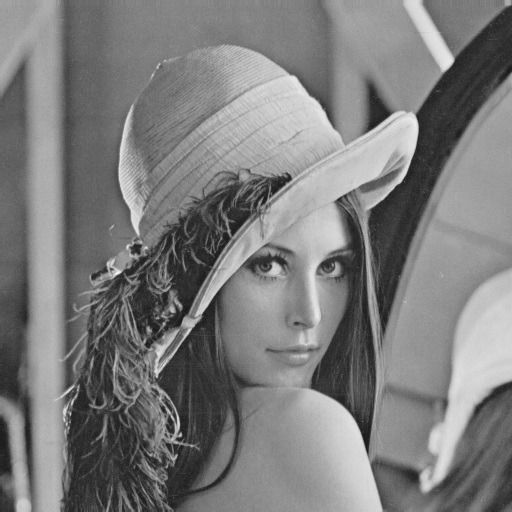
\includegraphics[width=.5\linewidth]{lenagrey}
  \captionof{figure}{Imagem original.}
\end{minipage}%
\begin{minipage}{.5\textwidth}
  \centering
  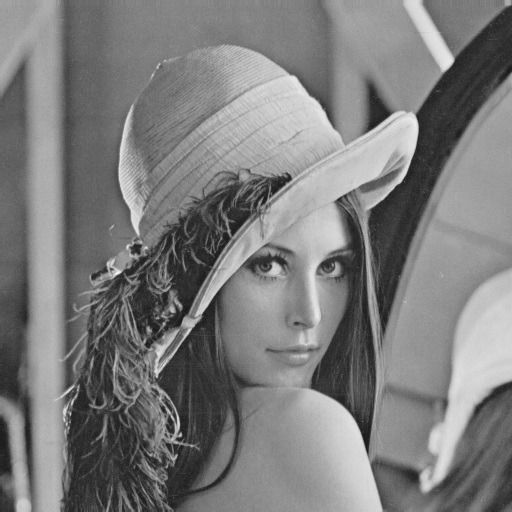
\includegraphics[width=.5\linewidth]{lenagrey}
  \captionof{figure}{Imagem descodificada.}
\end{minipage}
\end{figure}
\newpage

\section{Conclusões}
Com a finalização do trabalho foram obtidos conhecimentos acerca de técnicas com compressão sem perdas (\textit{Lossless}). Estas técnicas permitem fazer uma recuperação total dos dados após a compressão e devido a isso é obtida uma baixa taxa de compressão. Foram também estudados conceitos como a quantidade de bits necessária para representar um símbolo, entropia de fonte, número médio de bits por símbolo e eficiência do código. Os resultados obtidos estão dentro do que era suposto observar tirando o facto de apenas ter sido utilizada um tipo de média para teste do compressor desenvolvido.

\end{document}